\documentclass[10pt]{article}
\usepackage{icmlko}

\icmlmeta{IP 파운데이션 월드모델}{251}{반만 주면 다른 약이다}{공유 열을 일부 도메인에만 주면 그것은 절반이 아니라 \emph{전용 열}이다 --- 교차항의 정체}

\begin{document}

\twocolumn[
\icmlheader

\begin{abstract}
노트 250은 계수를 나눠 쓰는 자리에서 교차항이 부분합만큼 크다는 것을 쟀다
(1.01 대 0.18). 그 노트가 남긴 첫 물음 --- \textbf{나무도 같은 병인가.}
F18 배깅은 계수가 없고 문턱을 나눠 쓴다. 쟀더니 \textbf{같다}(공유 1.00 ·
분리 0.62). 선형 계수의 문제가 아니라 \emph{나눠 쓰는 모수} 일반의 문제다.
그런데 표를 보다가 더 이상한 것을 봤다 --- 공유 판에서 \textbf{전체 효과가
거의 정확히 0}인데(F18은 세 도메인 다 $\pm$0.0000) 부분들은 $\pm$0.01 씩
움직인다. 처음 짐작은 ``부분 적용이 도메인 깃발을 만든다''였다. \textbf{반증했다}:
마스크는 그대로 두고 값만 상수로 갈면 효과가 \textbf{정확히 0.0000} 이다 ---
원핫 절편이 이미 도메인을 나타내므로 깃발은 잉여다. 값을 잡음으로 갈면
$+$0.0023, 진짜 복사본이면 $+$0.0110 이다. \textbf{값이 하는 일이다.} 그러면
답은 하나뿐이다 --- \textbf{이름을 공유하는 열을 웹툰에게만 주면, 그 계수는
웹툰 행으로만 적합되므로 사실상 웹툰 \emph{전용} 열이다.} 실제로 그 값
($+$0.0110)이 노트 241이 잰 웹툰 전용 이름 열($+$0.0103)과 넷째 자리까지
같고, 전 도메인에 주면 $-$0.0003 으로 노트 241의 ``이름 공유''($+$0.0005)와
같다. \textbf{교차항은 결합이 아니었다.} ``혼자''와 ``남만''과 ``전체''가
같은 처치의 세 용량이 아니라 \textbf{서로 다른 세 처치}였던 것이다. 그래서
분해가 안 맞는 게 당연하다 --- 분해할 것이 애초에 없었다.
\end{abstract}
]

\section{나무도 같다}

노트 250은 능형(F21)으로만 쟀다. F18 배깅 트리는 계수가 없고 대신
\textbf{분할 문턱}을 아홉 도메인이 나눠 쓴다. 같은 실험을 형식마다 따로
돌렸다.

\begin{center}\small
\begin{tabular}{lrr}
\hline
 & 이름 공유 & 이름 분리 \\
\hline
F21 능형 & 1.01 & 0.42 \\
F18 나무 & \textbf{1.00} & 0.62 \\
\hline
\end{tabular}
\end{center}

같다. 그러니 노트 250이 ``계수''라고 쓴 것은 좁았다 --- \textbf{나눠 쓰는
모수}면 무엇이든 같다. 나무는 문턱을, 능형은 기울기를 나눠 쓴다.

\section{0 이 이상했다}

표를 다시 보다가 눈에 걸린 것은 비율이 아니라 \textbf{전체} 열이었다.

\begin{center}\small
\begin{tabular}{lrrr}
\hline
F18 · 이름 공유 & 합 & 전체 & 교차항 \\
\hline
웹툰 & $-$0.0003 & $\mathbf{+0.0000}$ & $+$0.0003 \\
애니 & $-$0.0060 & $\mathbf{+0.0000}$ & $+$0.0060 \\
게임 & $+$0.0143 & $\mathbf{+0.0000}$ & $-$0.0143 \\
\hline
\end{tabular}
\end{center}

전 도메인에 열을 더했는데 \textbf{아무 일도 안 난다}. 그런데 일부에게만
더하면 $\pm$0.014 씩 난다. 무언가가 ``일부''라는 사실 자체에서 나온다.

첫 짐작은 이랬다 --- 열을 웹툰에게만 주면 그 열의 \emph{관측 지표}가 웹툰
행에서 1, 나머지에서 0 이다. \textbf{도메인 깃발}이다. 전부에게 주면 그
지표가 상수라 죽는다. 노트 214의 가드 \textbf{한철}이 시간 축에서 잡아낸
바로 그 무늬가 도메인 축에서 난 것 아닌가.

\section{반증했다}

깃발 짐작은 값싸게 검정된다. \textbf{마스크는 그대로 두고 값만 간다.}
값이 상수면 깃발은 그대로인데 값은 아무것도 안 나른다.

\begin{figure}[t]
\centering
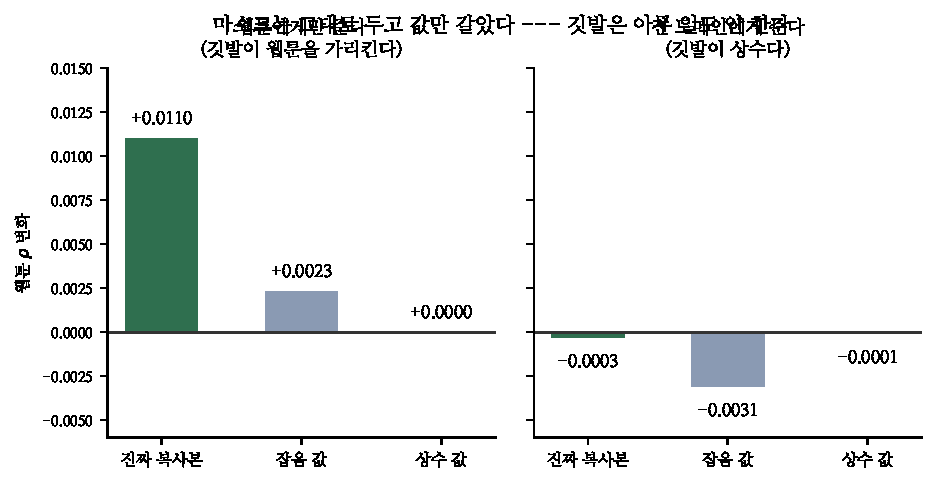
\includegraphics[width=\columnwidth]{figs/flag.pdf}
\caption{같은 마스크, 다른 값. 깃발이 살아 있는 왼쪽에서도 상수 값은
정확히 0 이다.}
\end{figure}

\begin{center}\small
\begin{tabular}{lrr}
\hline
값 & 웹툰에게만 & 전부에게 \\
\hline
진짜 복사본 & $+$0.0110 & $-$0.0003 \\
잡음 & $+$0.0023 & $-$0.0031 \\
\textbf{상수} & $\mathbf{+0.0000}$ & $-$0.0001 \\
\hline
\end{tabular}
\end{center}

\textbf{상수면 정확히 0 이다.} 깃발은 아무 일도 안 한다. 까닭은 노트 240이
이미 봤다 --- 한 도메인만 가진 축의 지표 열은 \textbf{그 도메인 원핫과 정확히
같고}(모바일에서 평균 1.000, 나머지 0.000), 원핫은 이미 설계행렬에 있다.
잉여 열은 능형에게든 나무에게든 새 정보가 아니다.

효과는 값에 있다. 잡음 값이 $+$0.0023, 진짜 값이 $+$0.0110 이다.

\section{반만 준 것이 아니라 다른 약이었다}

\begin{figure}[t]
\centering

\includegraphics[width=\columnwidth]{figs/same.pdf}
\caption{``일부에게 준 공유 열''과 ``전용 이름 열''이 같은 값을 낸다.}
\end{figure}

값이 하는 일이라면 남는 설명은 하나뿐이다. \texttt{dup\_tb} 라는 \emph{하나의}
이름을 웹툰에게만 주면, 그 계수는 웹툰 행으로만 적합된다. 이름은 공유인데
\textbf{내용은 웹툰 전용}이다. 노트 241이 정확히 그 물건을 따로 만들어 잰
적이 있다.

\begin{center}\small
\begin{tabular}{lr}
\hline
 & 웹툰 \\
\hline
이름 공유 열을 웹툰에게만 & $+$0.0110 \\
웹툰 \emph{전용} 이름 열 (노트 241) & $+$0.0103 \\[3pt]
이름 공유 열을 전 도메인에게 & $-$0.0003 \\
같은 열 · 이름 공유 · 판 전체 (노트 241) & $+$0.0005 \\
\hline
\end{tabular}
\end{center}

넷째 자리까지 맞는다. \textbf{``일부에게 준 공유 열''은 ``전용 열''이다.}

그러면 노트 249 · 250의 분해가 왜 안 맞았는지가 다르게 읽힌다. 나는
``혼자''와 ``남만''을 \emph{전체}라는 처치의 두 조각으로 여겼는데, 사실은

\begin{center}\small
\begin{tabular}{ll}
\hline
실험 & 실제로 무엇인가 \\
\hline
혼자 & 그 도메인에게 \textbf{전용} 열 하나 \\
남만 & 나머지 여덟에게 \textbf{그들끼리 공유}인 열 하나 \\
전체 & 아홉이 \textbf{진짜로 공유}하는 열 하나 \\
\hline
\end{tabular}
\end{center}

\textbf{서로 다른 세 처치다.} 셋을 더해서 안 맞는다고 ``교차항''이라 부른
것은 이름을 잘못 붙인 것이다. 교차항은 결합의 크기가 아니라
\textbf{내가 세 개의 다른 실험을 한 개의 분해로 읽은 오차}다.

\section{그래도 규약은 산다}

이름을 고쳤다고 실무가 바뀌지는 않는다. 오히려 더 단단해진다.

\begin{itemize}
\item 노트 249 · 250의 \emph{실용} 결론 --- ``공유 모수를 건드릴 때 도메인별
A/B 는 무효'' --- 은 그대로다. 이제 이유가 더 분명하다: 한 도메인에서 하는
시험은 \textbf{배포할 것과 다른 처치}이기 때문이다. 통계적 잡음이 아니라
\emph{다른 실험}이다.
\item 노트 239--242의 축 추가는 전용 이름이었으므로 여전히 유효하다.
\item 새로 얻은 것: \textbf{``이름을 공유하되 일부에게만''은 설계상 존재하지
않는 중간이다.} 그것을 만들면 전용 열이 된다. 그러니 축을 설계할 때 고를 것은
둘뿐이다 --- 전 도메인 공유냐, 도메인 전용이냐.
\end{itemize}

\paragraph{남은 것}
\begin{center}\small
\begin{tabular}{ll}
\hline
갈래 & 왜 \\
\hline
잡음 값 $+$0.0023 & 상수는 0 인데 잡음은 왜 양수인가 \\
``남만'' 처치 & 여덟이 그들끼리 공유하는 판. 쓸 데가 있나 \\
손 축 다섯 & 지금 유일한 진짜 공유. 전용으로 바꾸면 $-$0.031(노트 241) \\
웹툰 부호 갈림 & 남이 바꾸면 $+$0.035(노트 249) --- 아직 안 갈랐다 \\
\hline
\end{tabular}
\end{center}

\paragraph{규약} 분해 실험을 적을 때 \textbf{세 팔이 같은 처치의 세 용량인지
먼저 확인한다.} 공유 모수에서는 아니다 --- ``일부에게만''이 구조를 바꾼다.
아니면 ``교차항''이라는 말을 쓰지 말고 \textbf{세 실험을 따로 보고}한다.

\end{document}
